%%
%% This is file `sample-acmlarge.tex',
%% generated with the docstrip utility.
%%
%% The original source files were:
%%
%% samples.dtx  (with options: `acmlarge')
%% 
%% IMPORTANT NOTICE:
%% 
%% For the copyright see the source file.
%% 
%% Any modified versions of this file must be renamed
%% with new filenames distinct from sample-acmlarge.tex.
%% 
%% For distribution of the original source see the terms
%% for copying and modification in the file samples.dtx.
%% 
%% This generated file may be distributed as long as the
%% original source files, as listed above, are part of the
%% same distribution. (The sources need not necessarily be
%% in the same archive or directory.)
%%
%%
%% Commands for TeXCount
%TC:macro \cite [option:text,text]
%TC:macro \citep [option:text,text]
%TC:macro \citet [option:text,text]
%TC:envir table 0 1
%TC:envir table* 0 1
%TC:envir tabular [ignore] word
%TC:envir displaymath 0 word
%TC:envir math 0 word
%TC:envir comment 0 0
%%
%%
%% The first command in your LaTeX source must be the \documentclass command.
\documentclass[acmlarge]{acmart}
\usepackage{listings}
\lstset{language=Go,
  basicstyle=\ttfamily\scriptsize,
  keywordstyle=\color{blue}\ttfamily,
  stringstyle=\color{red}\ttfamily,
  commentstyle=\color{green}\ttfamily}
%%ss[STYLE]{acmart}
%% \BibTeX command to typeset BibTeX logo in the docs
\AtBeginDocument{%
  \providecommand\BibTeX{{%
    \normalfont B\kern-0.5em{\scshape i\kern-0.25em b}\kern-0.8em\TeX}}}

%% Rights management information.  This information is sent to you
%% when you complete the rights form.  These commands have SAMPLE
%% values in them; it is your responsibility as an author to replace
%% the commands and values with those provided to you when you
%% complete the rights form.
\setcopyright{acmcopyright}
\copyrightyear{2022}
\acmYear{2022}
\acmDOI{}


%%
%% These commands are for a JOURNAL article.
\acmJournal{POMACS}
\acmVolume{37}
\acmNumber{4}
\acmArticle{9}
\acmMonth{8}

%%
%% Submission ID.
%% Use this when submitting an article to a sponsored event. You'll
%% receive a unique submission ID from the organizers
%% of the event, and this ID should be used as the parameter to this command.
%%\acmSubmissionID{123-A56-BU3}

%%
%% The majority of ACM publications use numbered citations and
%% references.  The command \citestyle{authoryear} switches to the
%% "author year" style.
%%
%% If you are preparing content for an event
%% sponsored by ACM SIGGRAPH, you must use the "author year" style of
%% citations and references.
%% Uncommenting
%% the next command will enable that style.
%%\citestyle{acmauthoryear}

%%
%% end of the preamble, start of the body of the document source.
\begin{document}

%%
%% The "title" command has an optional parameter,
%% allowing the author to define a "short title" to be used in page headers.
\title{Paper Reading of \textit{CloudScale: Elastic Resource Scaling for Multi-Tenant Cloud Systems}}

%%
%% The "author" command and its associated commands are used to define
%% the authors and their affiliations.
%% Of note is the shared affiliation of the first two authors, and the
%% "authornote" and "authornotemark" commands
%% used to denote shared contribution to the research.
\author{Yiwei Yang}
\email{yangyw@shanghaitech.edu.cn}
\orcid{0000-0001-8011-5868}
\affiliation{
  \institution{ShanghaiTech University}
  \streetaddress{1 R.D. Zhongke}
  \city{Shanghai}
  \state{Shanghai}
  \country{China}
  \postcode{21210}
}

%%
%% By default, the full list of authors will be used in the page
%% headers. Often, this list is too long, and will overlap
%% other information printed in the page headers. This command allows
%% the author to define a more concise list
%% of authors' names for this purpose.
\renewcommand{\shortauthors}{Yiwei Yang}

%%
%% The abstract is a short summary of the work to be presented in the
%% article.
\begin{abstract}
  In Infrastructure as a Service provider uses virtualizations to provide isolation among users. CloudScale \cite{shen2011cloudscale}, as an adaptive augmentation to the IaaS, is a multi-tenant cloud computing infrastructure resource scaling technology that automates fine-grained elastic resource scaling. CloudScale achieves adaptive resource allocation without assuming any prior knowledge of the applications running inside the cloud by using online resource demand prediction and prediction error management.
\end{abstract}
%%
%% The code below is generated by the tool at http://dl.acm.org/ccs.cfm.
%% Please copy and paste the code instead of the example below.
%%
\begin{CCSXML}
  <ccs2012>
  <concept>
  <concept_id>10010520.10010553.10010562</concept_id>
  <concept_desc>Distributed System~Peer to Peer System</concept_desc>
  <concept_significance>500</concept_significance>
  </concept>
  </ccs2012>
\end{CCSXML}

\ccsdesc[500]{Distributed System~Service Level Objective~Serverless}

%%
%% Keywords. The author(s) should pick words that accurately describe
%% the work being presented. Separate the keywords with commas.
\keywords{}


%%
%% This command processes the author and affiliation and title
%% information and builds the first part of the formatted document.
\maketitle
\section{Strong point of the document}
\subsection{In a prediction-driven resource scaling system, CloudScale uses sophisticated strategies - predictive migrations to limit SLO breaches.}
\begin{figure}[H]
  \centering
  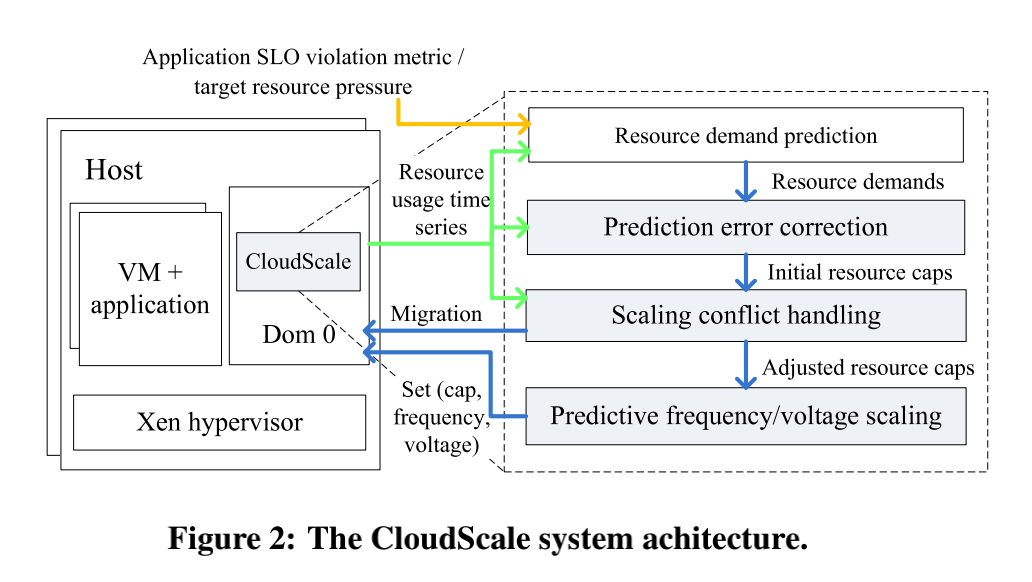
\includegraphics[width=10cm]{./overview.png}
\end{figure}
Once the SLO violation is triggered, the prediction will start whether to migrate based on the VM Xen's memory usage and system's CPU usage. The prediction will also examine on other error and scaling conflicts.
\subsection{Minimized under-estimation errors}
To avoid under-estimation correction, the proactive approach is Burst-based Padding, which is a signal processing, called reverse FFT on resource usage time series and calculate the metrics burst density metrics.
\begin{figure}[H]
  \centering
  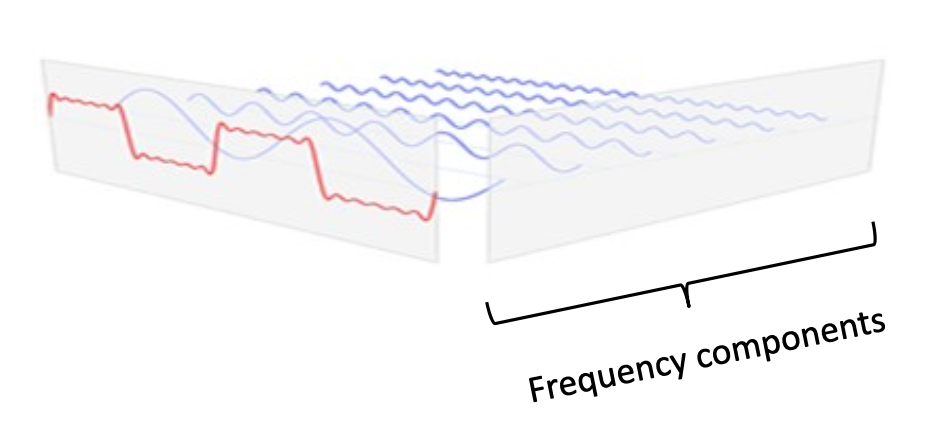
\includegraphics[width=10cm]{./prediction.png}
\end{figure}
Here's the Padding values decided according to the extracted burst pattern.
\begin{figure}[H]
  \centering
  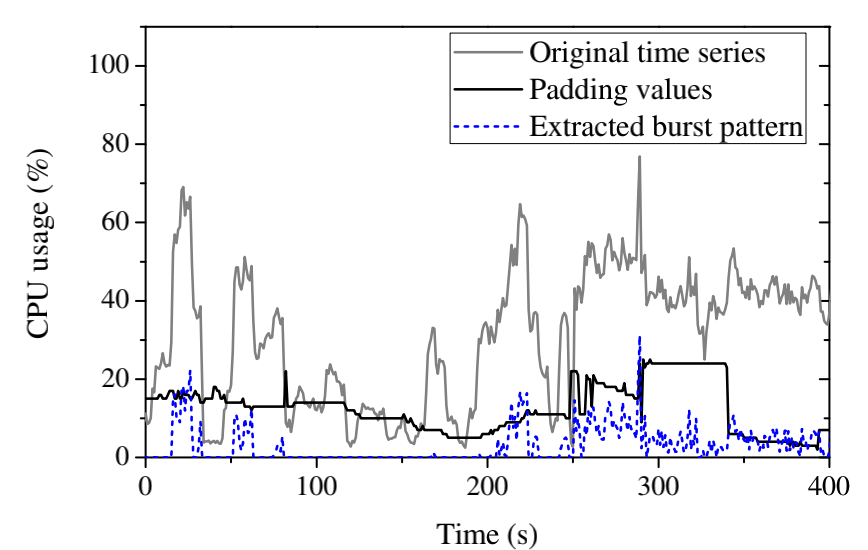
\includegraphics[width=10cm]{./pattern.png}
\end{figure}
\subsubsection{Resource Demand Prediction}
\begin{figure}[H]
  \centering
  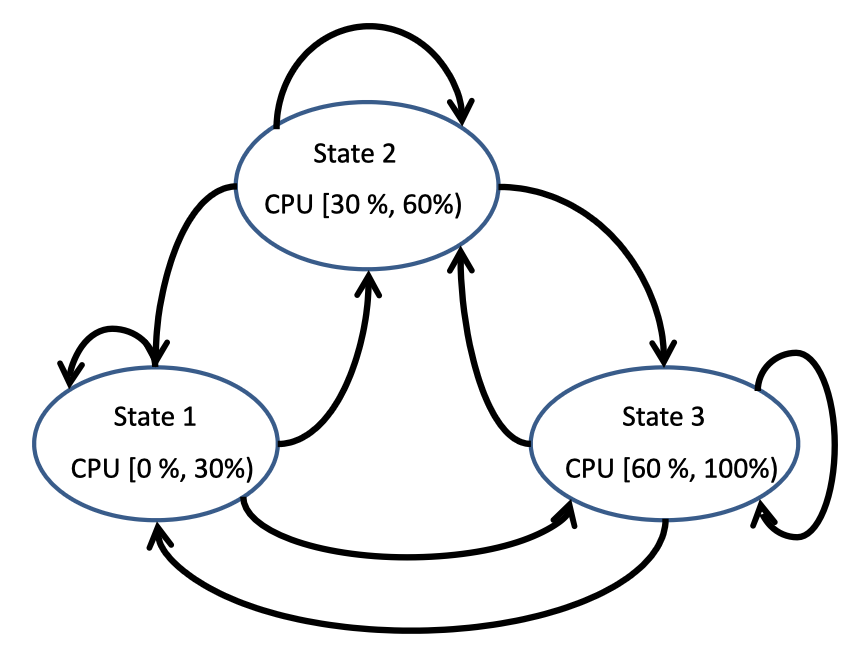
\includegraphics[width=10cm]{./resource_demand.png}
\end{figure}
\begin{enumerate}
  \item State-driven resource demand prediction.
  \item used when no signature is found.
\end{enumerate}

\subsubsection{Prediction Error Correction}
\begin{figure}[H]
  \centering
  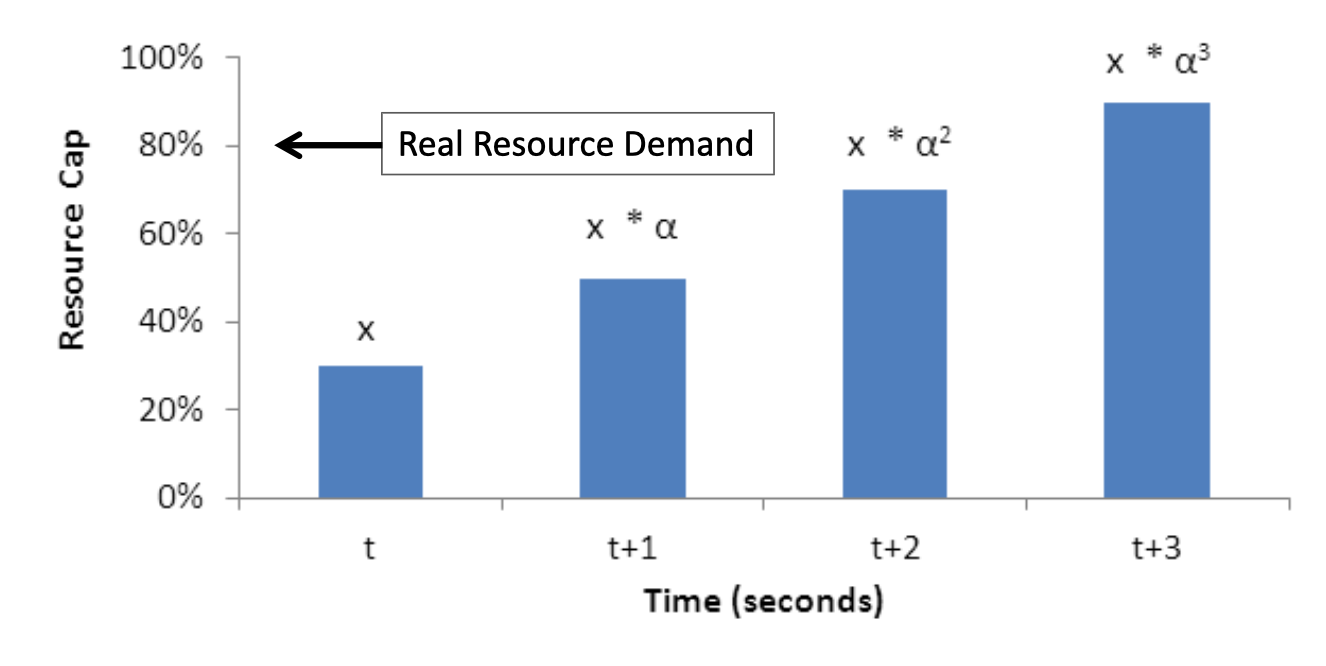
\includegraphics[width=10cm]{./error_correction.png}
\end{figure}
\begin{enumerate}
  \item The correction uses fast under-estimation Correction.
  \item The challenge is real resource demand is unknown during under-provisioning.
\end{enumerate}
The threshold is defined for pressure calculation, and once the ratio is upper than predefined 75\%, it will carry out the correction.
\begin{figure}[H]
  \centering
  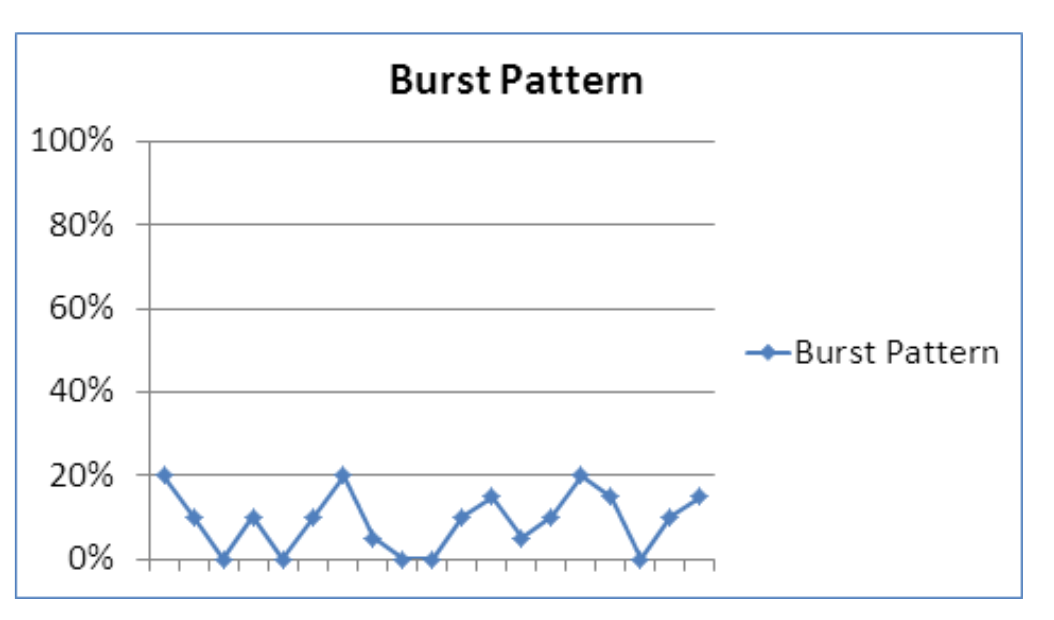
\includegraphics[width=10cm]{./burst.png}
\end{figure}

\section{Scaling Conflict Handling}
\subsection{Conflict Prediction}
For each VM, the scaling system has a long-term resource demand forecast model. In contrast to the resource scaling system's prediction model, which utilizes a 1-second prediction interval, the long-term prediction model uses a 10-second prediction interval to forecast further into the future.

To reduce the total penalty, CloudScale assigns resources depending on application priorities or resource under-provisioning penalties of distinct apps.
\subsection{Scale based on the voltage and frequency}
CloudScale combines virtual machine resource scaling with dynamic voltage and frequency scaling to turn wasted resources into energy savings while keeping application SLOs intact. For example, if resource demand prediction models show that a host's overall CPU resource demand is 50\%, we can reduce the CPU frequency and increase the resource caps for all application VMs. As a result, we can save energy because the CPU is running at a lesser speed, but the application's SLO is unaffected.
\section{Weak point of the document}
\subsection{The isolation of multi-tenancy is not well considered}
The prediction on the frequency may let the malicious attacker utilize the metrics to occupy the resources for one time.
\subsection{IO operations and GPU metrics should also be take into account}
By \cite{kim2015towards}, we know that the IO metrics are very important for the prediction for multi-tenant Cloud Systems, especially when the guest OS is running a IO intensive application.
\section{Possible Refinement}
\subsection{Add more metrics to the prediction}
The network flow, IO flow and GPU metrics can be added to the burst pattern analysis.
\subsection{Add shim and disaggregation for better protection and cost-efficiency}
The isolation for Xen is not enough to maintain isolation and cost-efficiency in nowadays Virtual Machine. One we applies a shim and disaggregation, we can utilize metrics from shim to implement the same logic as CloudScale.
\bibliographystyle{ACM-Reference-Format}
\bibliography{cloudScale_elastic_resource_scaling_for_multi_tenant_cloud_systems}
\end{document}
\endinput
%%
%% End of file `sample-acmlarge.tex'.
